\documentclass{article}
\usepackage[margin=1in]{geometry}
\usepackage{array}
\usepackage{graphicx}
\usepackage{natbib}

\author{Carl Ehrett}
\title{Computer model calibration as a method of design}

\begin{document}

\maketitle

\section{Introduction}
% Discussion of computer experiments and computer model calibration. Lit review. Overview of project goals.

\subsection{Computer experiments}

Suppose that one wishes to improve one's understanding of, say, the movement of people in a crowd escaping from a building in a crisis situation. This is an example of an area in which field data are extremely difficult to acquire. Merely assembling a crowd of research subjects in one place is costly and difficult. Asking them to flee a building may result in behaviors which are unlike those in real crisis situations -- but which may nonetheless present unacceptable physical risk to the subjects. Inducing them to flee through the generation of a (real or apparent) crisis is similarly infeasible. Observational data are likewise scarce here, since panic-inducing crises are by their nature difficult to predict and chaotic in ways that hinder the reliable collection of data.

In the face of these difficulties, computer models offer an alternative to the choice between attempting field data collection and giving up on the hope of progress. Using existing theory concerning human psychology and movement, it is possible to construct a computer model simulating the behavior of people evacuating from a large building. For example, the SIMULEX model described by \cite{Thompson1995} allows one to observe simulated evacuation behaviors in any specified building layout, using any desired physical distribution of individuals, whose individual relevant characteristics (walking speed, initial bodily orientation, etc) may be controlled by the researcher. Thus, computer models provide a means to collect data which might otherwise be largely inaccessible. 

The study of computer models from a statistical perspective calls for specialized tools and techniques. Gaussian processes (GPs) are a popular tool for modeling the output of computer code. There are three reasons for this popularity: (1) The use of a GP does not require detailed foreknowledge of the approximate parametric form of the computer model. Researchers often lack such foreknowledge in the case of complex computer models. (2) GPs easily interpolate the observed data. This is an advantage when the observations come from deterministic computer code that is free of observation error. (3) The variance of a GP provides a natural form of uncertainty quantification. 
A Bayesian approach to the study of computer models is undertaken by \cite{Currin1991}; the authors approach GPs as prior distributions on the unknown form of the computer model. A frequentist applications of GPs to computer models is provided by \cite{Sacks1989}, who use GPs not only for estimating uncertainty but also as the basis for their approach to experimental design in the area of deterministic computer models.  \cite{Santner2003a} offer a comprehensive discussion of to the use of GPs for prediction, design, and sensitivity analysis with respect to computer experiments from both frequentist and Bayesian perspectives.

\subsection{Computer model calibration}

Suppose that we wish to use the SIMULEX model to compare two different proposed building codes to be enforced in, say, St.\ Louis, Missouri. We may use average walking speed and average interpersonal distance as input parameters for this model, both to settle the initial physical distribution of people throughout the building and to influence their behavior during evacuation. It is well-established that average walking speed \citep{Bornstein1976} and interpersonal distance \citep{Sorokowska2017} vary across locales. These values may be unknown for the case of St.\ Louis. Thus we may wish to find the true values for average walking speed and interpersonal distance in St.\ Louis; we may wish, in other words, to \textit{calibrate} these parameters in the model.

Broadly, in model calibration, we may consider a model to be of the form $\eta(x,\theta)$, where $(x,\theta)$ comprise all inputs to the model. Control inputs --- inputs under the control of the researcher (in the evacuation example, this would include the building layout) comprise $x$, whereas $\theta$ is the set of calibration inputs --- parameters the values of which are not under researcher control, but rather are unknown values which must be estimated for successful simulation. Thus where $f$ describes the true system, we consider the model to be 
\begin{equation}f(x,\theta)=f(x)=\eta(x,\theta) + \delta(x)
\end{equation} where $\delta$ describes the model discrepancy -- i.e., the bias of the model as an estimate of the real system. Notice that we may write $f(x)=f(x,\theta)$ since $\theta$ does not vary in reality. To undertake model calibration, we must have access to at least some observations of the real system; it is to these real observations that we calibrate the computer model.

Much interest in the past two decades has centered on Bayesian methods for model calibration. The appeal of a Bayesian approach to model calibration lies in the fact that the calibration parameters are a source of uncertainty for the model. This uncertainty should be quantified so that its effect on the model can be made explicit. We can thus use Bayesian methods to arrive at a posterior distribution on the calibration parameters which balances our prior knowledge about the calibration parameters with what can be learned from the available data, and which also allows for accurate uncertainty quantification on the model outputs. The work of \cite{Kennedy2001} has been influential in this area. Kennedy and O'Hagan offer a Bayesian approach to computer model calibration that allows for the uncertainty of the calibration parameters in the predictions of the resulting calibrated model. 

\subsubsection{Gaussian processes}

\paragraph{Background}



\paragraph{Gaussian process regression}

\begin{figure}[h]
\centering
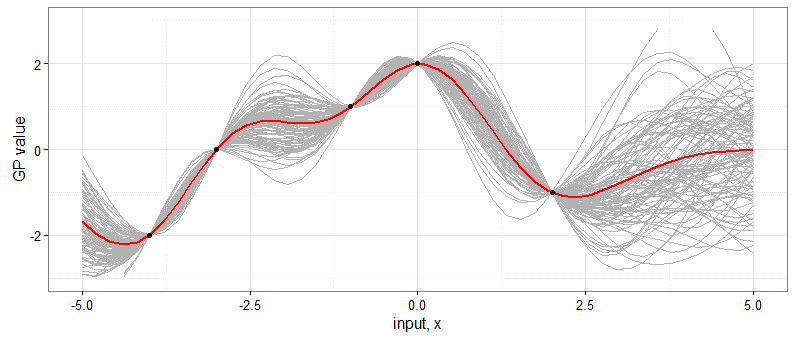
\includegraphics[width=.75\linewidth]{gp_example}
\caption{Example of a Gaussian process trained to interpolate five data points (black dots).}
\label{gp_example}
\end{figure}

\paragraph{Gaussian processes in computer model calibration}

\subsubsection{Markov chain Monte Carlo methods}

\paragraph{Background}

\paragraph{Metropolis-Hastings algorithm}

\paragraph{Elimination of boundary constraints}

\subsubsection{Normalization of inputs and standardization of outputs}
Blah

\subsubsection{Computational difficulties}
% And solutions
Blah

\paragraph{Likelihoods}
Blah

\paragraph{Ill-conditioned covariance matrices}

\section{Calibration for design}



\section{Application}

\subsection{Project background}

\subsection{Emulation of finite element simulator}
Blah

\subsubsection{Wind turbine blade simulator}
% Here the finite element model will be described
Blah

\subsubsection{Mathematical basis for the emulator}
% Includes formulae for trained mean and covariance functions
Blah

\subsubsection{Experimental design}
% How we selected the design points at which to observe the simulator
Blah

\subsubsection{Covariance parameters}
% How they were selected
Blah

\paragraph{Finding covariance parameters via MCMC}
% Why we didn't do it (computational difficulties
Blah

\paragraph{Grid optimization}
% Advantages and disadvantages; full grid and integration of lambda
Blah

\paragraph{Gradient method}
% Explanation and advantages
Blah

\begin{figure}
\centering
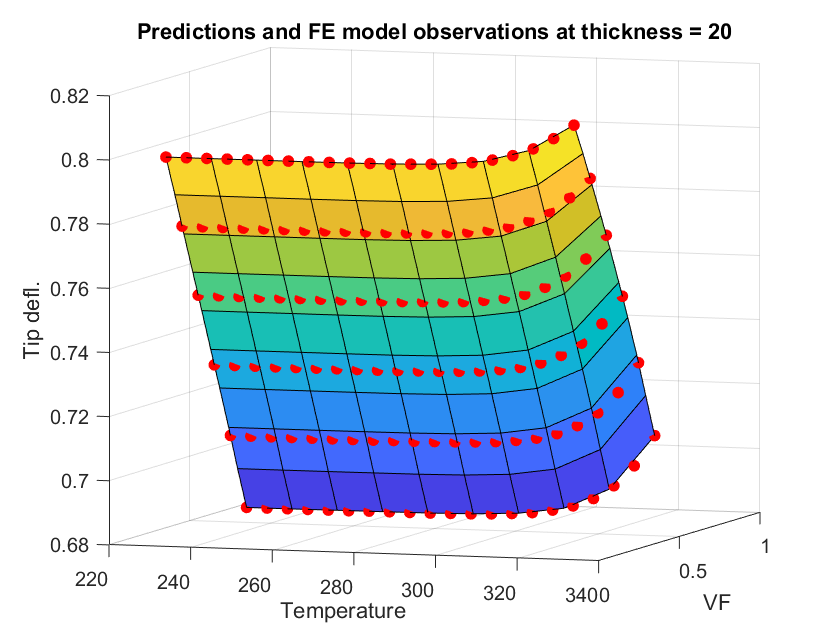
\includegraphics[width=.65\linewidth]{emulator_surface}
\caption{A slice of the GP emulator (restricted to the output for tip deflection) at thickness =20mm. Red dots are observations from the simulator.}
\label{fig:emulator_surface}
\end{figure}

\section{MCMC using the emulator}
Blah

\subsection{MCMC methods}
% Background on MCMC
Blah

\subsection{The model}
% Choice of priors and resulting likelihood
Blah

\subsubsection{Desired observation variance}
% 4 versions: heterosked constant, homosked constant, heterosked prior, homosked prior
\begin{table}[h]
\centering
\begin{tabular}{| c | c  |  c  | c |  c  |}
\hline
 \vspace{-3mm}
& & & & \\
& \parbox{24mm}{\centering Heteroskedastic, constant}& \parbox{24mm}{\centering Homoskedastic, constant}& \parbox{24mm}{\centering Heteroskedastic, prior} & \parbox{24mm}{\centering Homoskedastic, prior}\\
 \vspace{-3.5mm}
& & & & \\
\hline
Deflection & 0.749 & 0.729 & 0.659 & 0.709\\
Rotation & 0.0904 & 0.0865 & 0.0773 & 0.0843\\
Cost & 276.16 & 236.11 & 350.80 & 233.95 \\
\hline
\end{tabular}
\caption{Comparison of model outputs, where the desired data outputs are assumed to be either homoskedastic or heteroskedastic, with either a specified constant variance or a $1/\sigma^2$ prior.}
\label{table:obs_var_comp}
\end{table}

\begin{figure}
\centering
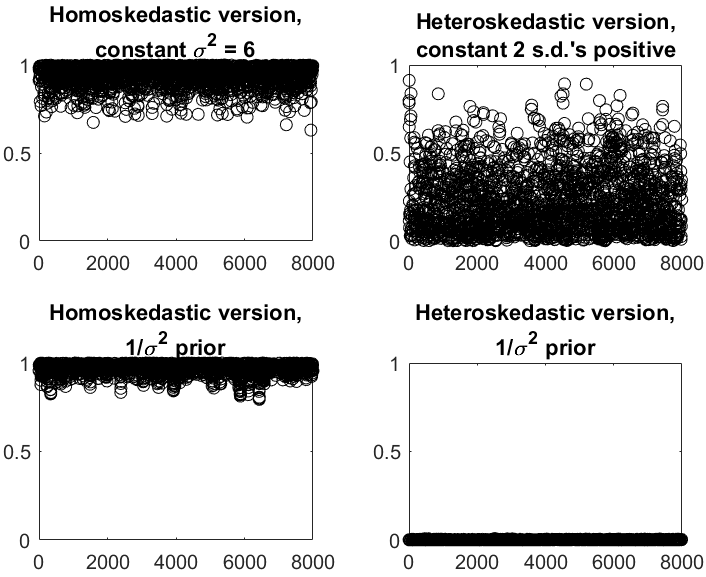
\includegraphics[width=.65\linewidth]{comp_obs_var}
\caption{MCMC results at various observation variance settings.}
\label{fig:comp_obs_var}
\end{figure}

\subsubsection{Full model and likelihood}
Blah

\subsubsection{Convergence difficulties}
% And the idea to eliminate boundary constraints
Blah

\subsubsection{Implementation of the Metropolis-Hastings algorithm}
Blah

\begin{figure}
\centering
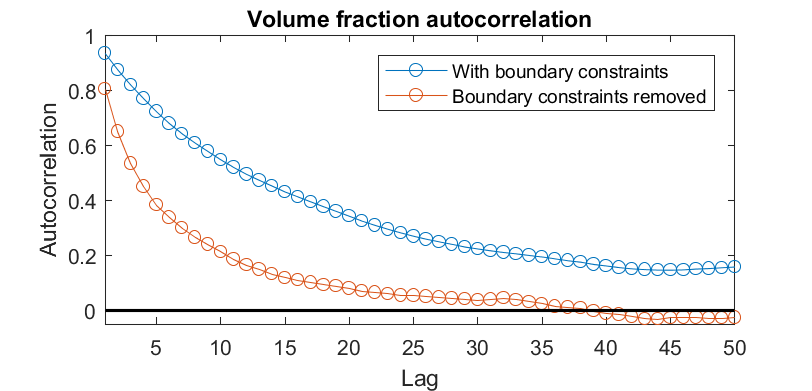
\includegraphics[width=.9\linewidth]{ACF_bnd_cnds_fig}
\caption{Auto-correlation for draws both with and without the elimination of boundary conditions.}
\end{figure}

\subsection{Which data to desire?}
Blah

\subsubsection{Motivations behind the choice of desired data}
Blah

\subsubsection{Differing results}
% for different desired data values
\begin{table}[h]
\centering
\begin{tabular}{| c | c  | c  |  c | c  | c | c | c |}
\hline
Desired data $d$ & $\sigma^2_{defl}$ & $\sigma^2_{rot}$ & $\sigma^2_{cost}$ & $\mu_{v|d}$ &
                            $\mu_{h|d}$ & $\sigma^2_{v|d}$ & $\sigma^2_{h|d}$\\
\hline
$(0, 0, 0)$ & 375.45 & 277.69 & 2.62 & 0.215 & $4.01 \cdot 10^{-2}$&
	$4.41\cdot 10^{-2}$ & $1.92 \cdot 10^{-3}$\\
$(0.65, 0.077, 96)$ & 16.74 & 15.25 & $4.62 \cdot 10^{-7}$ &
	$1.09 \cdot 10^{-3}$ & $3.36 \cdot10^{-4}$ &
	$1.02 \cdot 10^{-5}$ & $9.97 \cdot 10^{-6}$\\
\hline
\end{tabular}
\caption{Comparison of results for two different (low) values of $d$. Values listed are, respectively, the posterior means for the observation variance of each model output, posterior means for volume fraction ($v$) and thickness ($h$), and posterior variance of volume fraction and thickness.}
\label{table:d_comp}
\end{table}

\begin{figure}
\centering
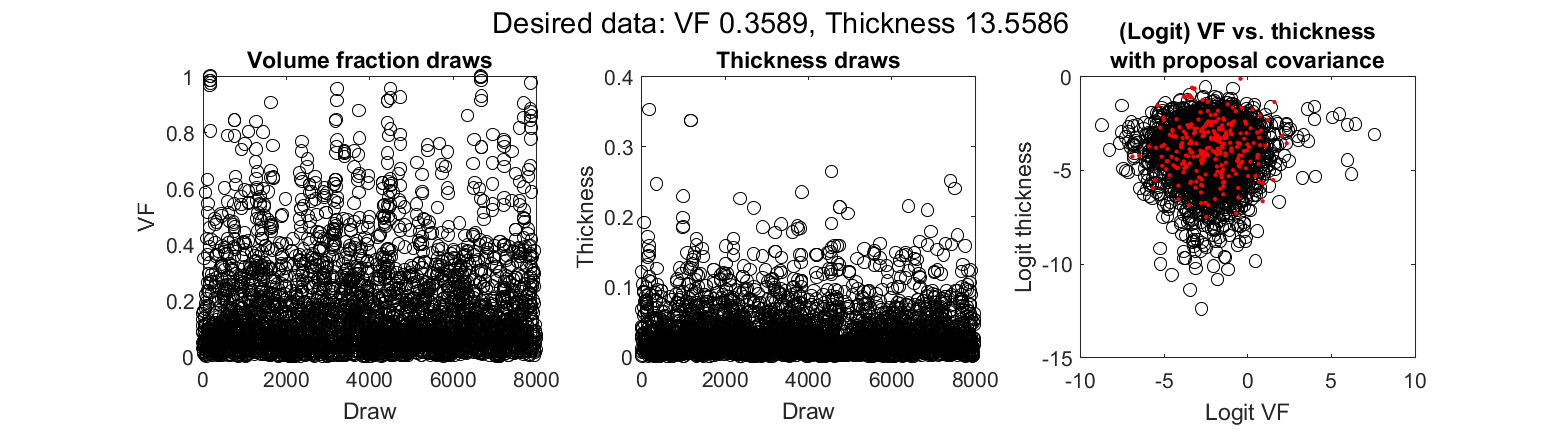
\includegraphics[width=.9\linewidth]{FIG1}
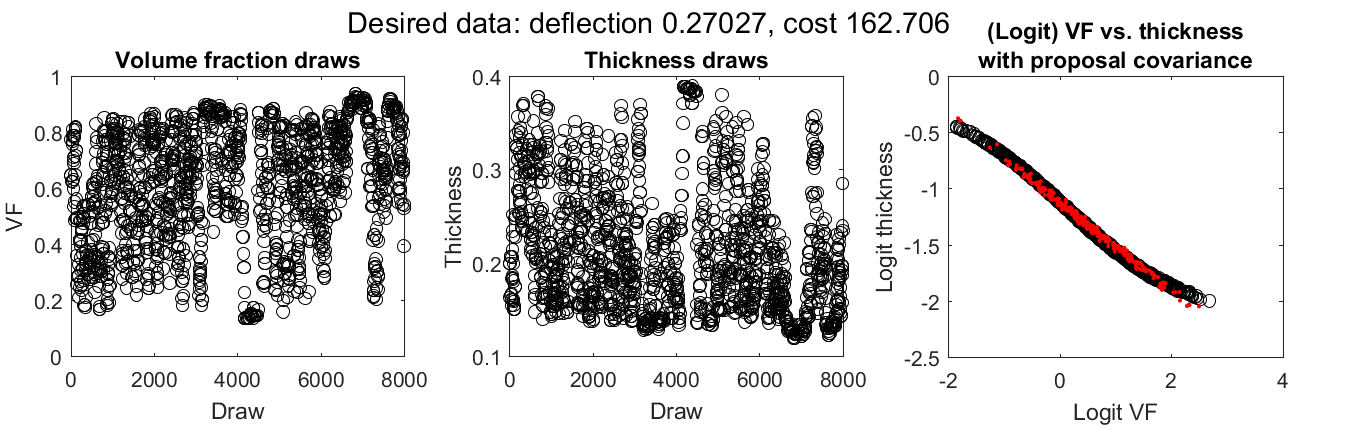
\includegraphics[width=.9\linewidth]{FIG2}
\caption{MCMC results for low deflection and cost (top row) and low deflection with easily achievable cost (bottom row).}
% NOTE: THESE PLOT TITLES ARE WRONG! GOTTA DO THE PLOTS OVER! LOL!
\label{fig:des_data}
\end{figure}

\subsection{Exponentially distributed desired data}
Blah

\subsubsection{Motivation}
Blah

\subsubsection{Implementation and results}
Blah


\subsection{Identifiability issues}
% Issues arising from the non-identifiability of VF, thickness when cost is relaxed
Blah

\section{Future work}
Blah

\subsection{Alternative means of handling cost}
Blah

\subsubsection{Removing cost from the model}
Blah

\subsubsection{Alternative priors for controlling cost}
Blah

\subsection{Building a desired data response surface}
Blah

\subsection{Implementing Hamiltonian Monte Carlo}
Blah

\subsubsection{Hamiltonian Monte Carlo}
% Background
Blah

\subsubsection{Benefits}
Blah

\subsection{Model discrepancy}
% Include (or investigate the inclusion of) a model discrepancy function
Blah

\section{Conclusion}
% Discussion of the role of computer model validation as a potential methodology for design
Blah












\bibliographystyle{authordate1}
% This style file is a version of the plain.bst style file which I edited myself to add abstract and annotation fields.

\bibliography{lit_review}

\end{document}